\documentclass[12pt]{beamer}

\usetheme{Frankfurt}
\setbeamercolor{structure}{fg=orange}
\setbeamertemplate{footline}[frame number]

\usepackage{tikz}
\usetikzlibrary{positioning}

\usepackage{animate}
\usepackage{epstopdf}


\hyphenpenalty=10000

\title{Data-Driven Methods for the Reduction \\of Multiscale Stochastic Data}

\author{Carmeline J. Dsilva}
\date{28 October 2014}

\begin{document}

\begin{frame}[plain]

\titlepage

\end{frame}

\section{Introduction}

\begin{frame}{Underlying Motivation}

Multiscale time series are ubiquitous

\end{frame}


\begin{frame}{Goals for Analysis}

Reduction

\end{frame}


\begin{frame}{How to Reduce?}

Model-driven reduction (singularly peturbed problem)

Data-driven reduction

\end{frame}

%\begin{frame}{Outline}
%
%\tableofcontents
%%\begin{itemize}
%%\item Multiscale SDE framework
%%\item Data reduction (diffusion maps)
%%\item Mahalnobis distance to capture relevant timescales
%%\item Examples
%%\item Conclusion/applications/future work
%%\end{itemize}
%
%\end{frame}


\section{Multiscale SDEs}

\begin{frame}{Multiscale Data}

\begin{equation*}
\begin{aligned}
dx_i(t) &= a_i(\vec{x}(t)) dt + dW_i(t), & \: 1 \le i \le m \\
dx_i(t) &= \frac{a_i(\vec{x}(t))}{\epsilon} dt + \frac{1}{\sqrt{\epsilon}} dW_i(t) , & \: m+1 \le i \le n
\end{aligned}
\end{equation*}

This SDE has $m$ slow variables and $n-m$ fast variables

Under some mild conditions, we can write a {\em reduced} SDE in {\em only} the slow variables $x_1, \dots, x_m$.

\end{frame}

\section{Data Reduction}

\begin{frame}{Data Reduction in General}

\begin{tikzpicture}

\node(a){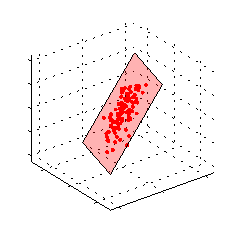
\includegraphics{PCA_3D}};
\node(texta)[below=0cm of a, text width=4cm, align=center] {High dimensional data on low-dimensional structure};
\node[right=2cm of a](b){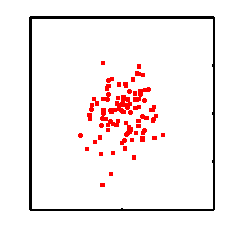
\includegraphics{PCA_2D}};
\node(texba)[below=0cm of b, text width=4cm, align=center] {Want to reduce dimensionality};
\draw[->] (a) -- (b);
\end{tikzpicture}

\end{frame}

\begin{frame}{Principal Component Analysis for Data Reduction}

{\bf Idea:} Find directions of maximum variance in data set

These directions should capture the ``important'' features of the data


\end{frame}

\begin{frame}{Diffusion Maps for Nonlinear Data Reduction}
    
    \begin{tikzpicture}
        \node (fig1) {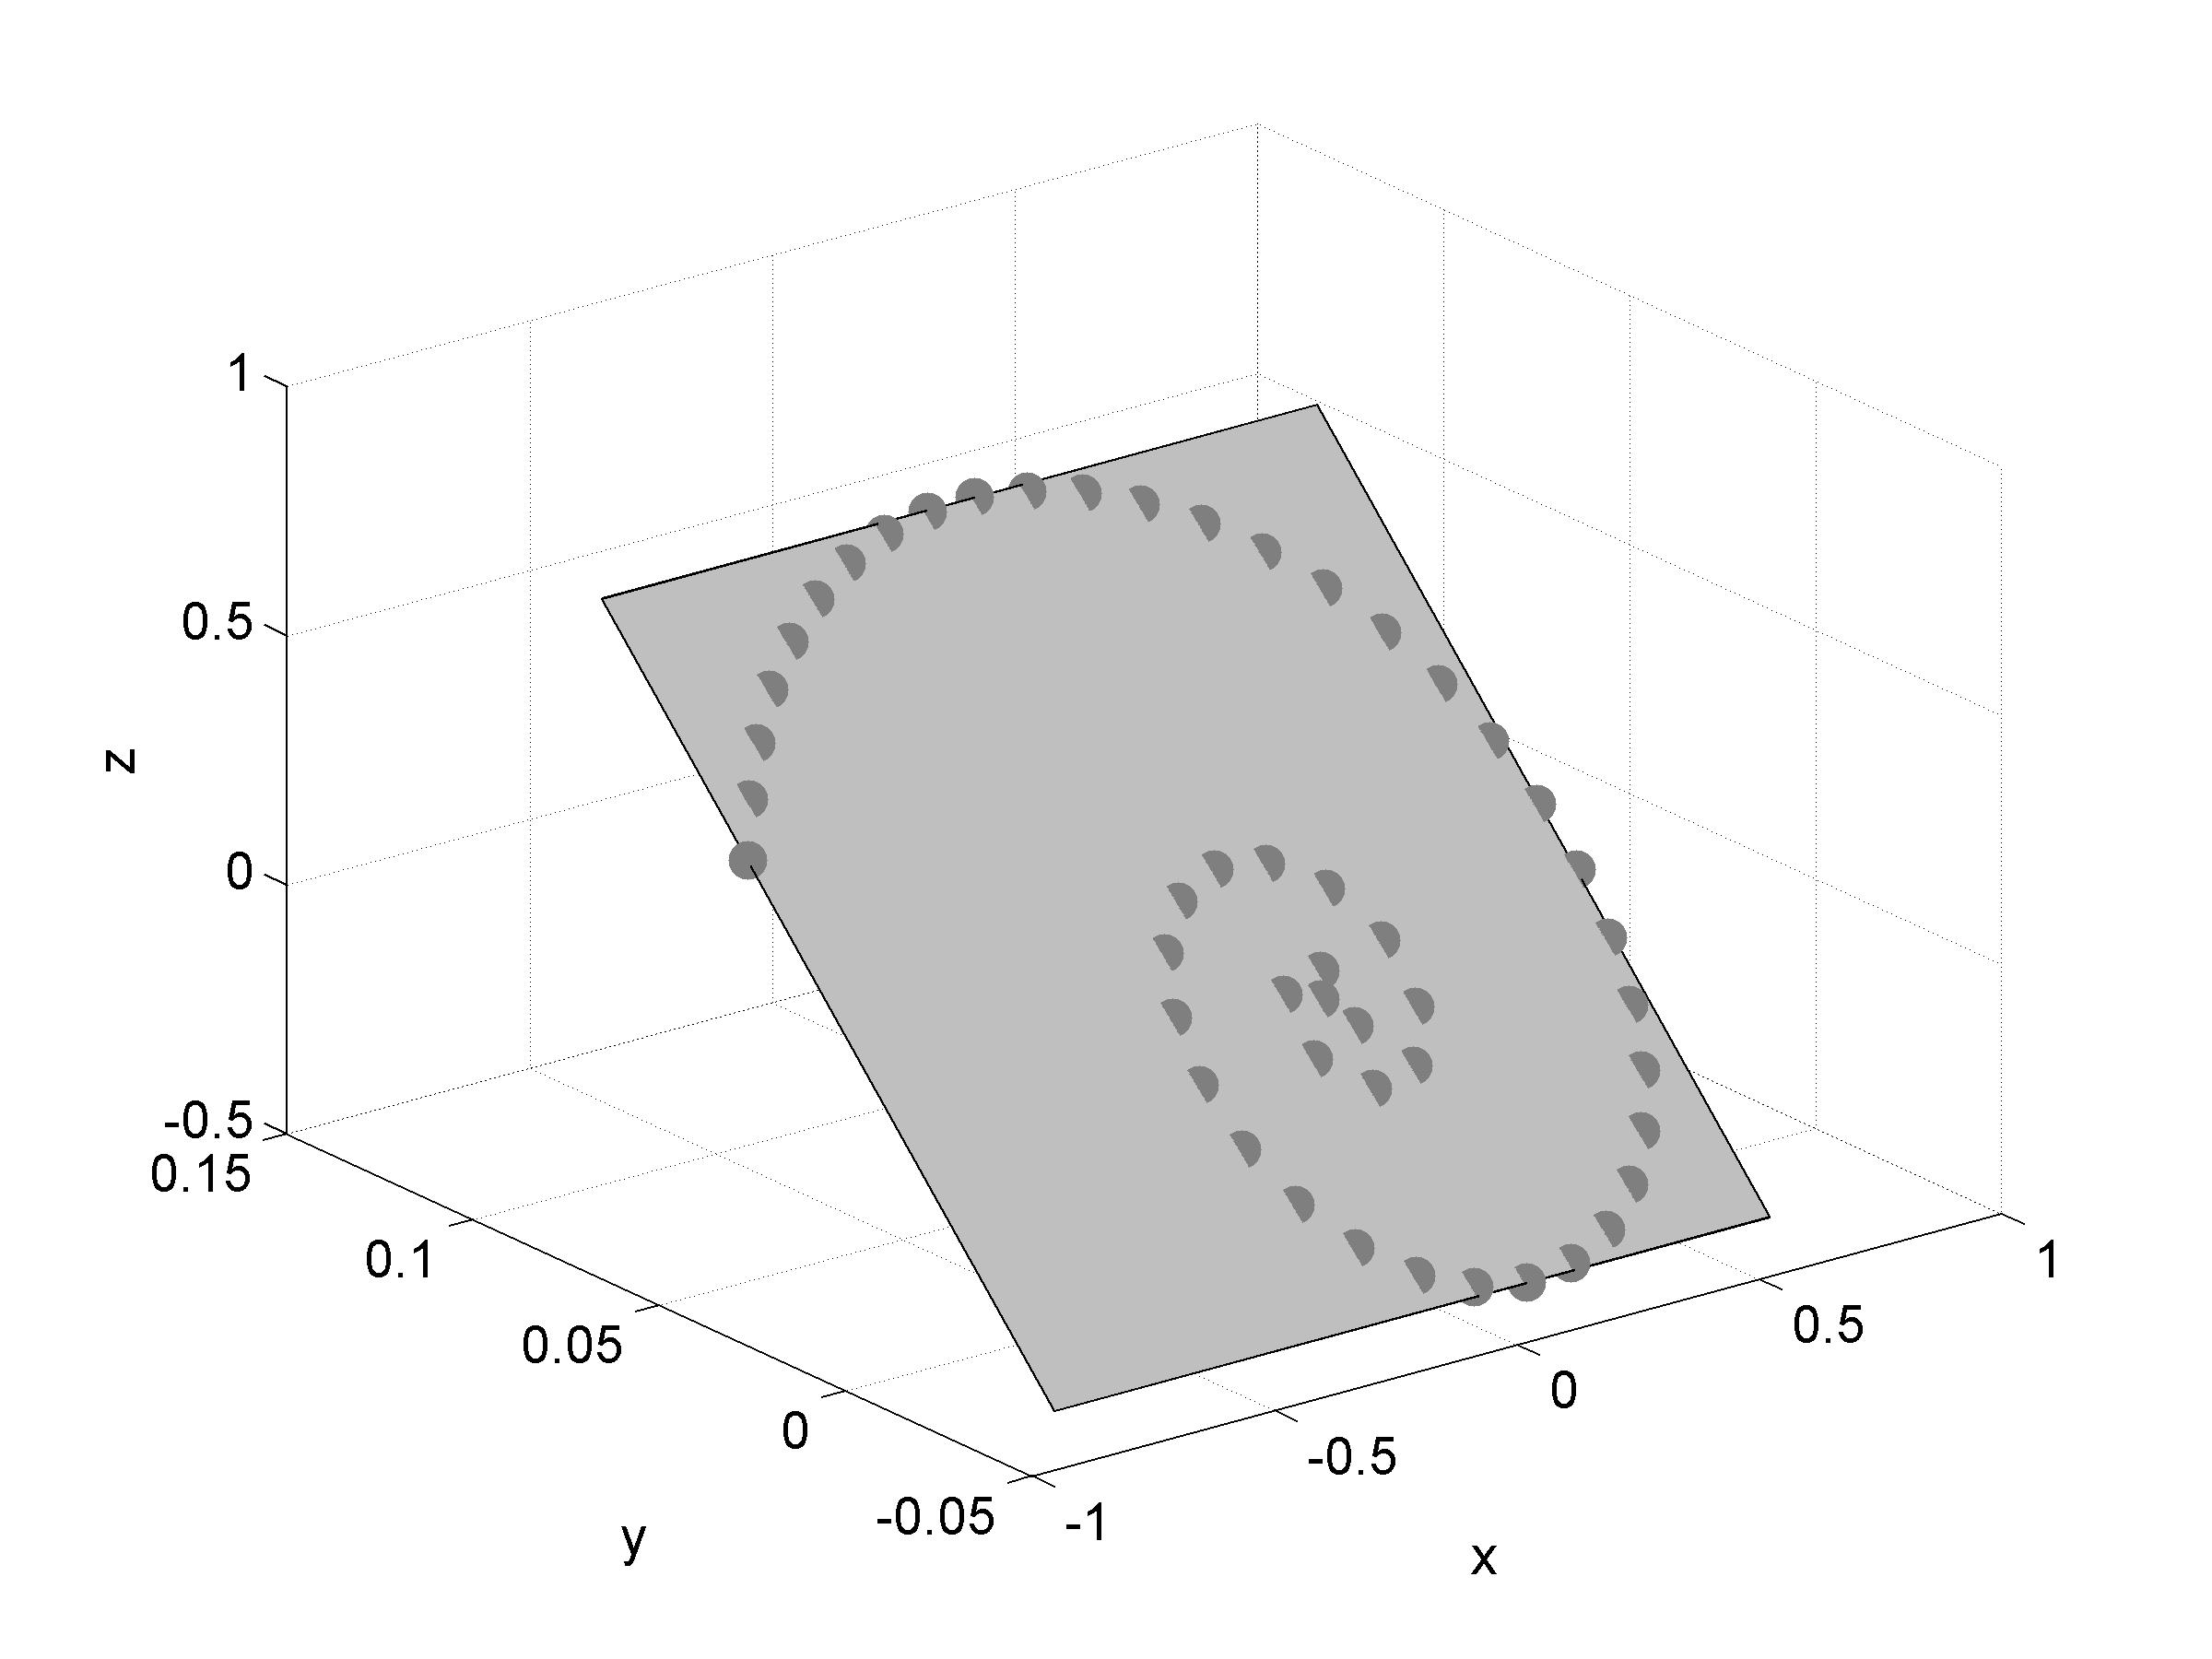
\includegraphics[width=0.3\textwidth]{dmaps_spiral_black_plane_large.jpg}};
        \draw[red,->] (-0.1,-0.95) -- (1, -0.68);
        \draw[red,->] (-0.1,-0.95) -- (-0.9, 0.5);
        \node[right of=fig1, node distance=0.5\textwidth] (fig2) {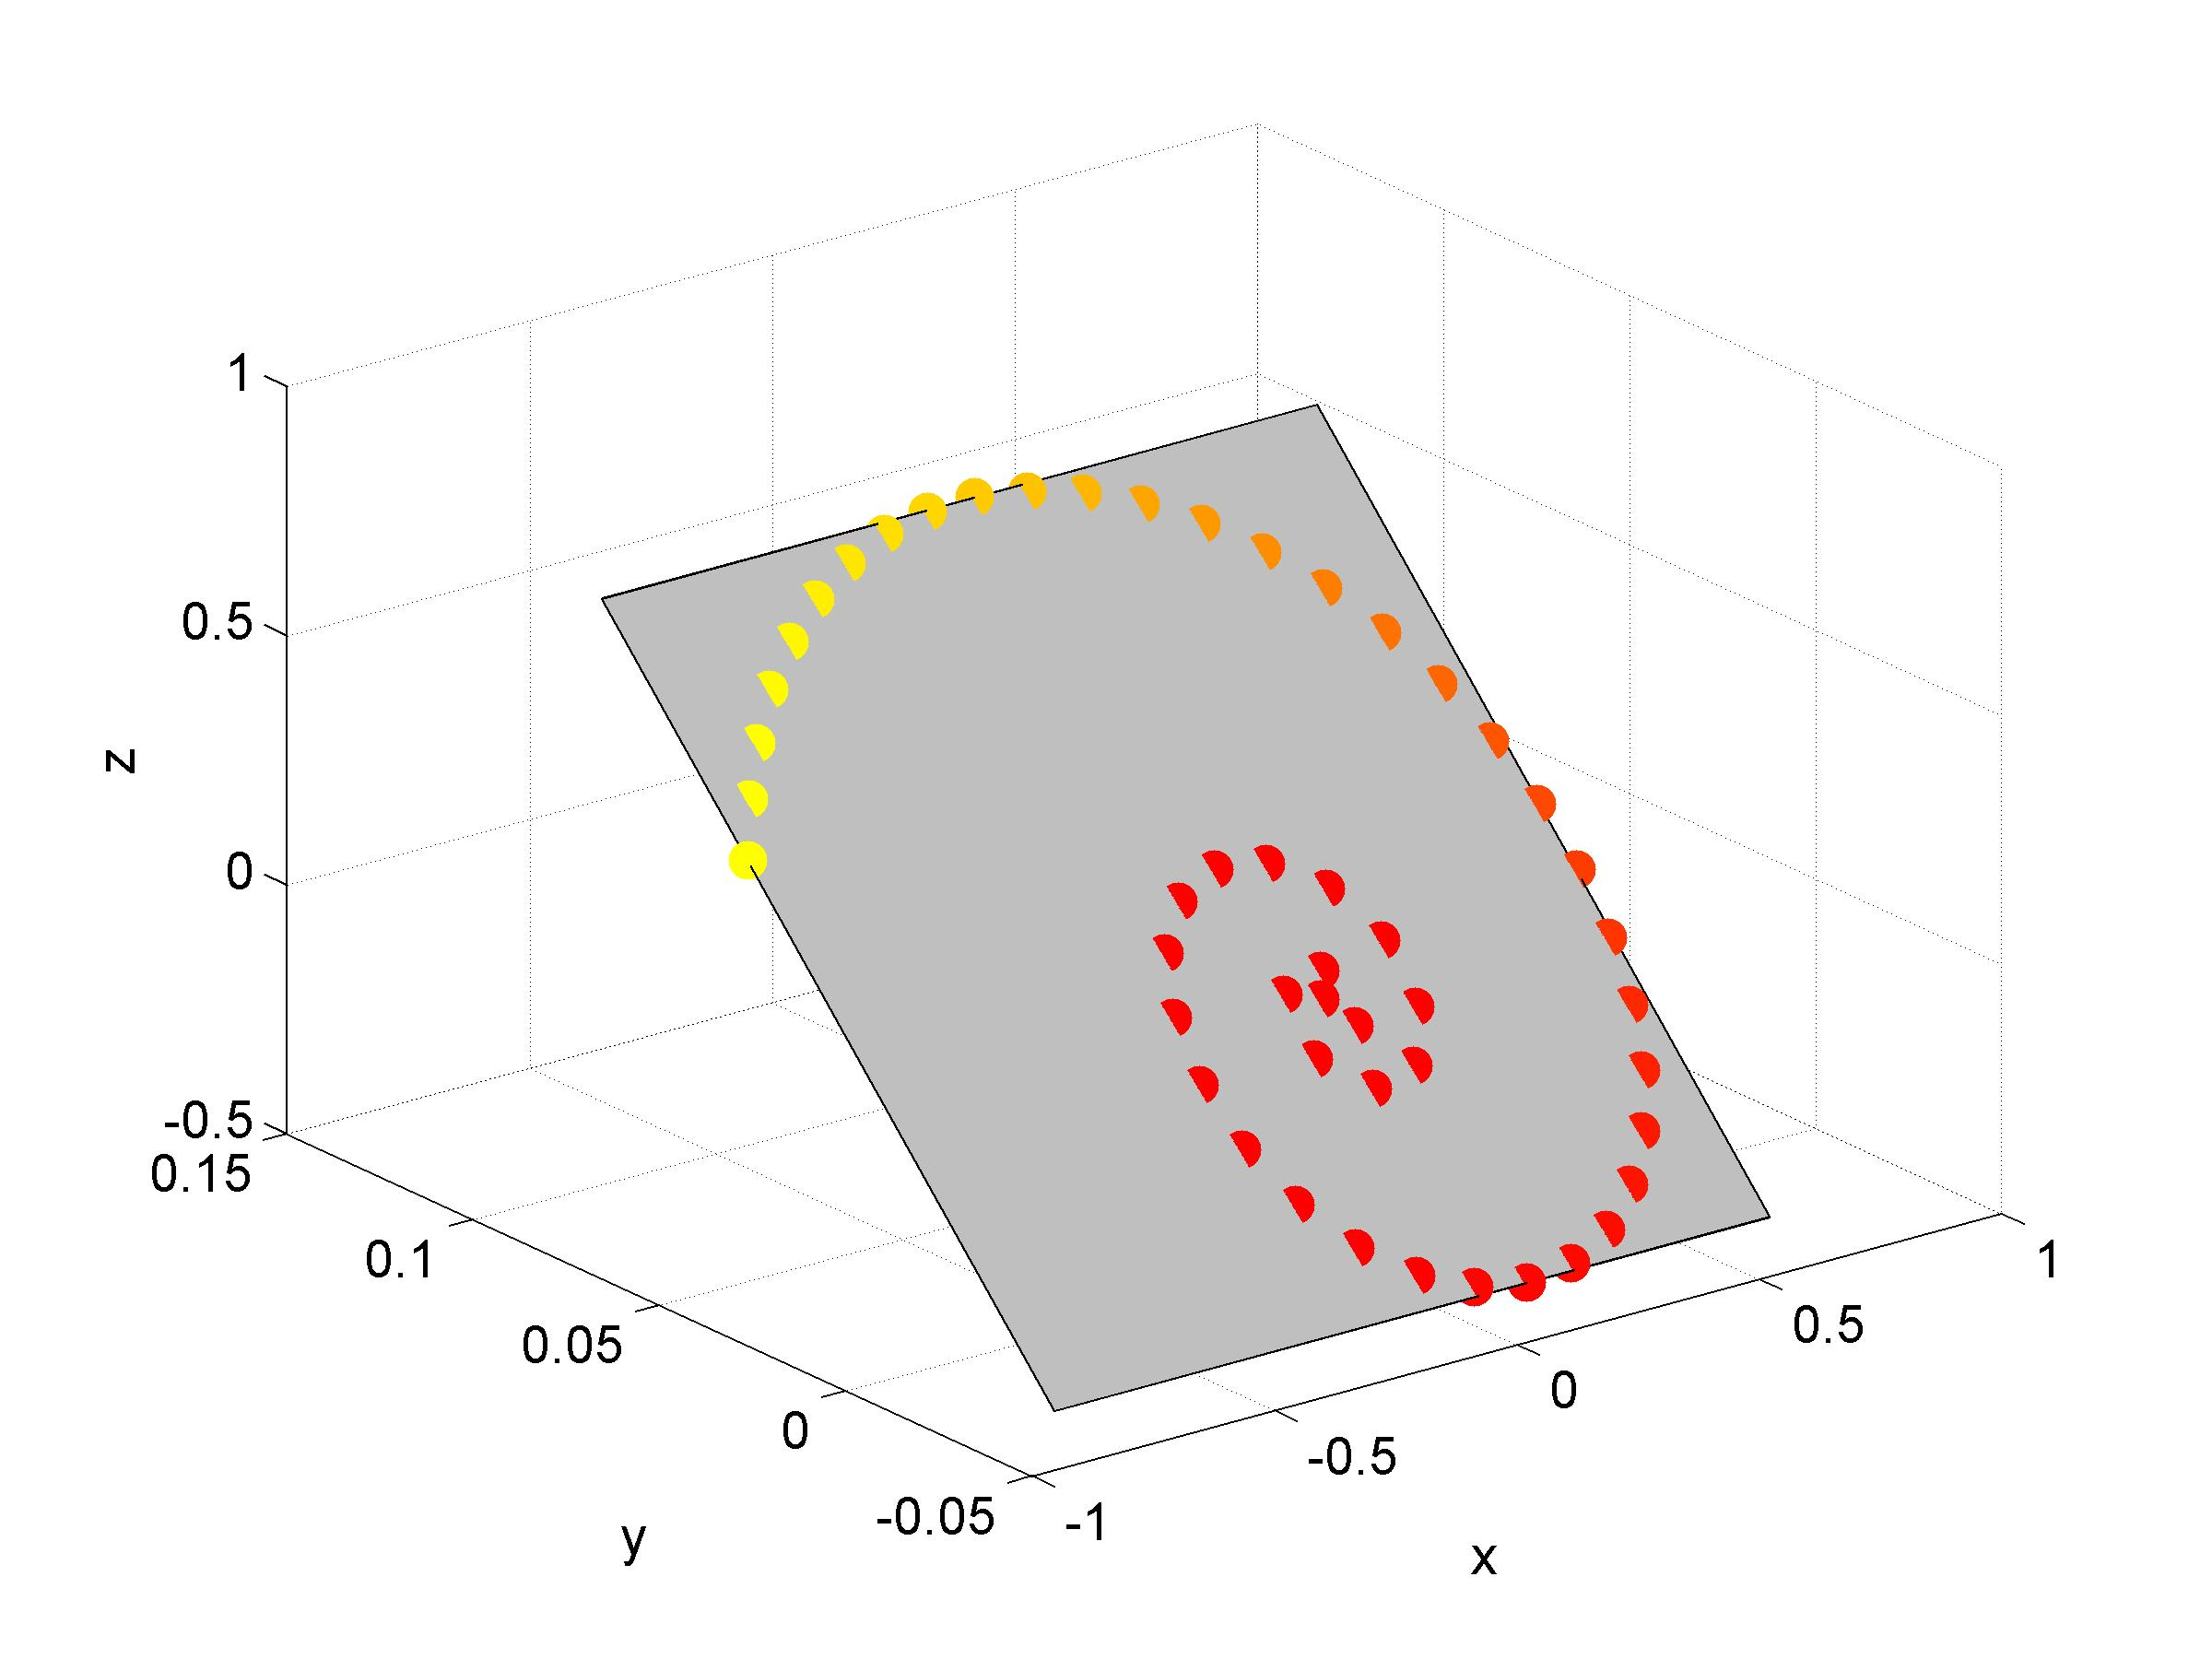
\includegraphics[width=0.3\textwidth]{dmaps_spiral_color_plane_large.jpg}};
        \draw [->] (fig1.east) -- (fig2.west);
    \end{tikzpicture}

	\vspace{-0.1in}
	{\scriptsize 
	On the left are data that lie on a spiral. 

	PCA will ``uncover'' a (two-dimensional) plane and give you a coordinate system (principal components). 

	On the right, the data have been colored by the first DMAPS coordinate. 

	DMAPS can ``uncover'' the one-dimensional {\em nonlinear manifold} and give you a coordinate system (arclength). \par }

\end{frame}

\begin{frame}{Eigenfunctions to Parameterize a Manifold}

    %\vspace{0.15in}
    {\scriptsize
    \begin{minipage}[t]{0.3\textwidth}
        \centering
        Consider a manifold\\
        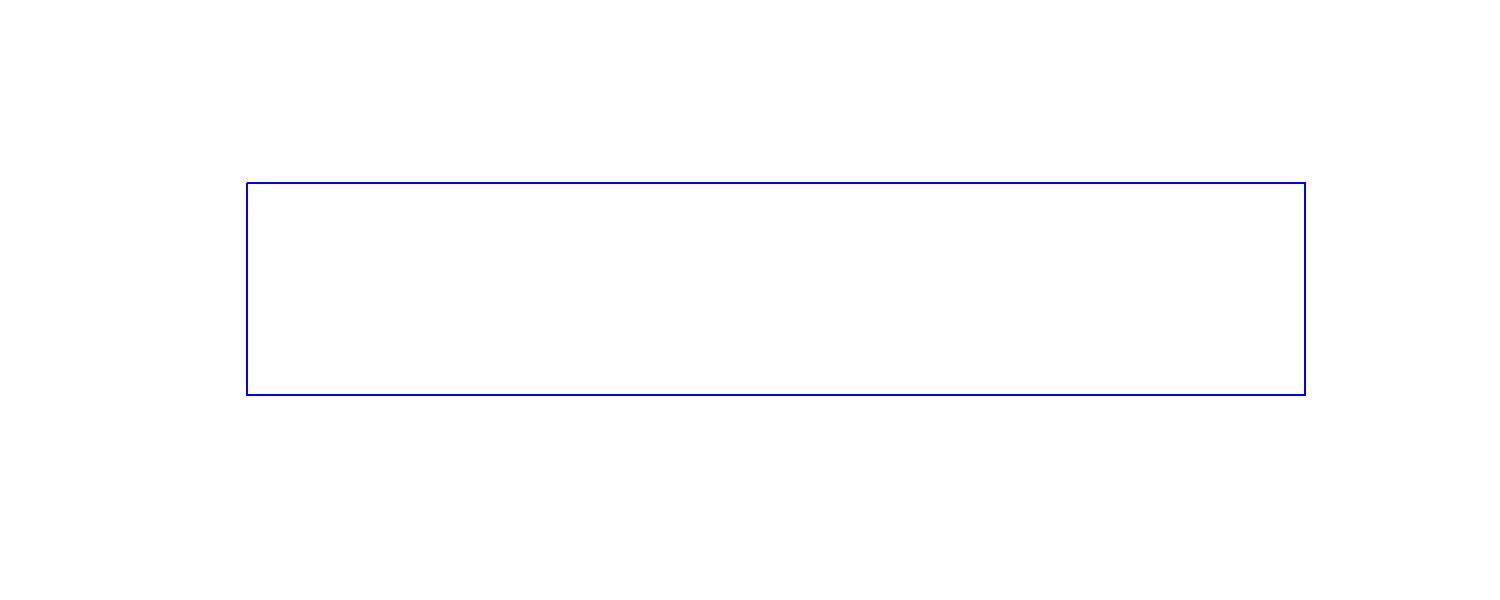
\includegraphics[width=\textwidth]{rect.jpg}\\


    \end{minipage}
    \begin{minipage}[t]{0.35\textwidth}
        \centering
        We want a ``good'' parametrization of~the manifold\\
        \vspace{0.1in}
        \animategraphics[width=\textwidth]{1}{rect_efunc}{1}{6}\\
        \vspace{-0.03in}
        These parameterizations are the~eigenfunctions of $\nabla^2 \phi$\\
    \end{minipage}
    \begin{minipage}[t]{0.3\textwidth}
        \centering
        Instead, we have data {\em sampled} from the manifold and want to~obtain a parameterization\\
        \vspace{0.1in}
        \animategraphics[width=\textwidth]{1}{rect_evec}{1}{6}\\
        \vspace{0.1in}
        We therefore {\em approximate} the~Laplacian on the data
    \end{minipage}
    \par}

    \vspace{0.1in}

    \centering
    {\small We obtain a similar parametrization for a curved manifold \par}
    \vspace{0.05in}
    
\includegraphics[width=0.18\textwidth]{circle.jpg}
    \hspace{0.03\textwidth}
    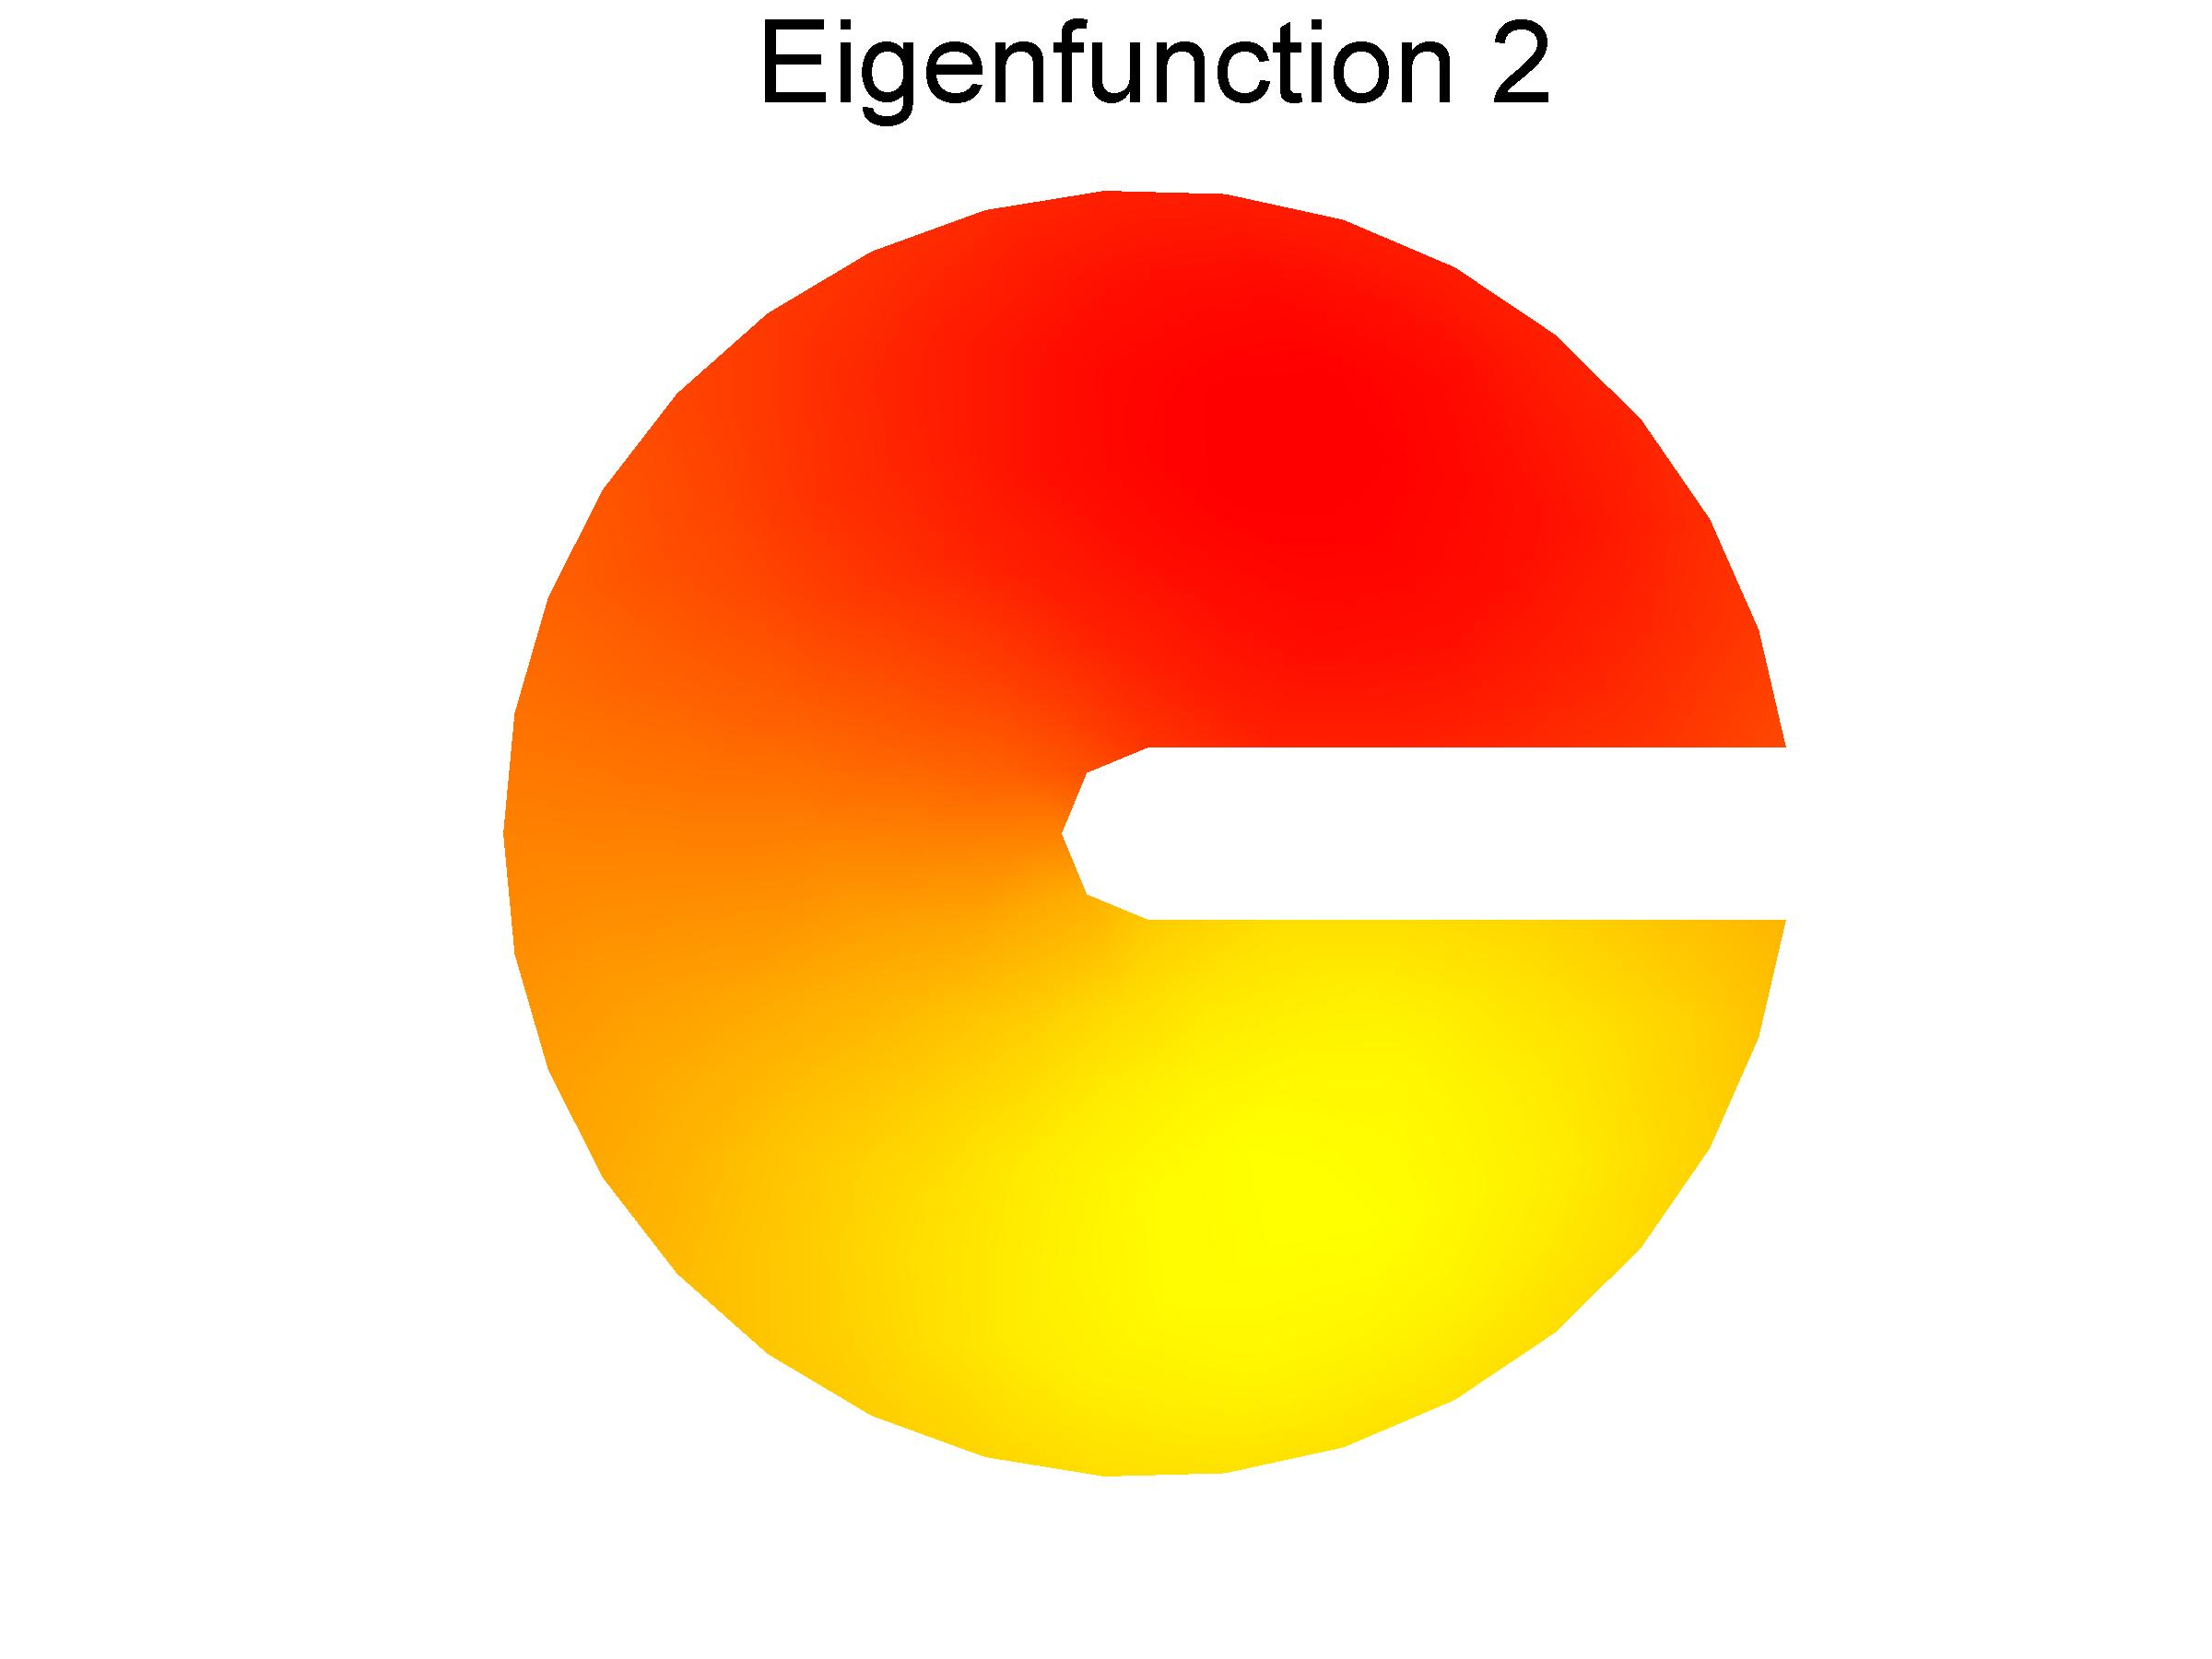
\includegraphics[width=0.18\textwidth]{circle_efunc1.jpg}
    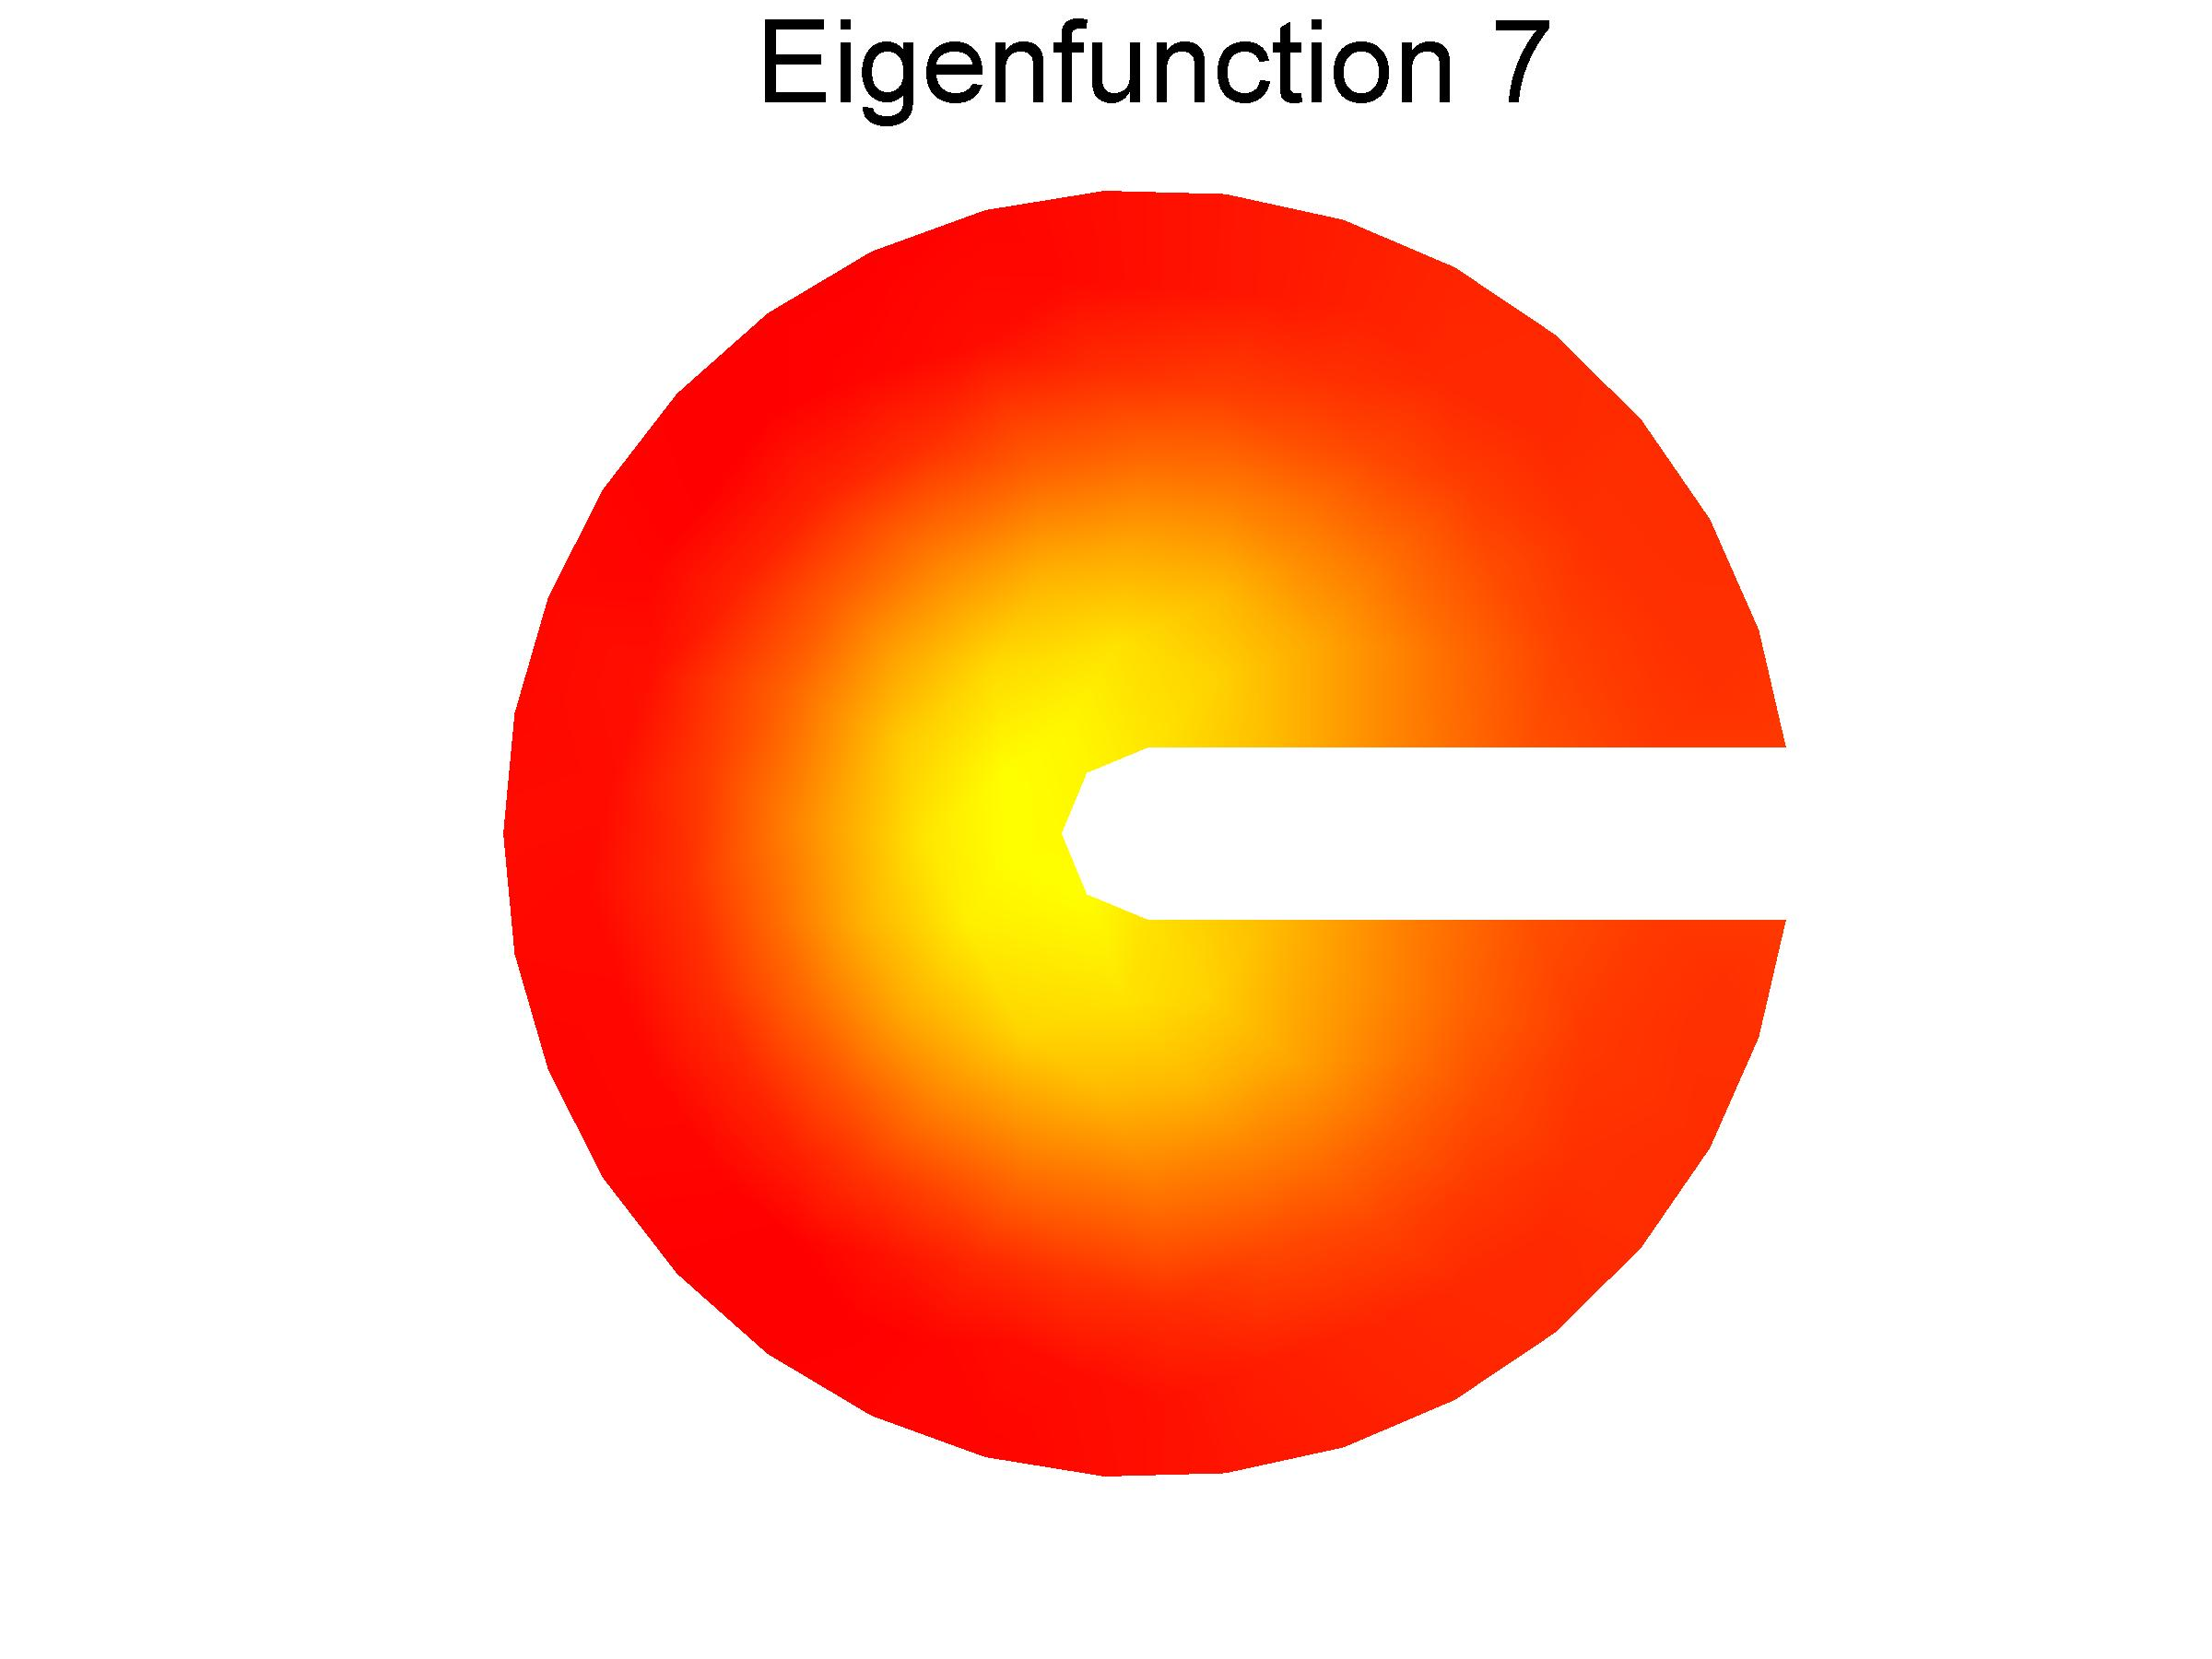
\includegraphics[width=0.18\textwidth]{circle_efunc6.jpg}
    \hspace{0.03\textwidth}
    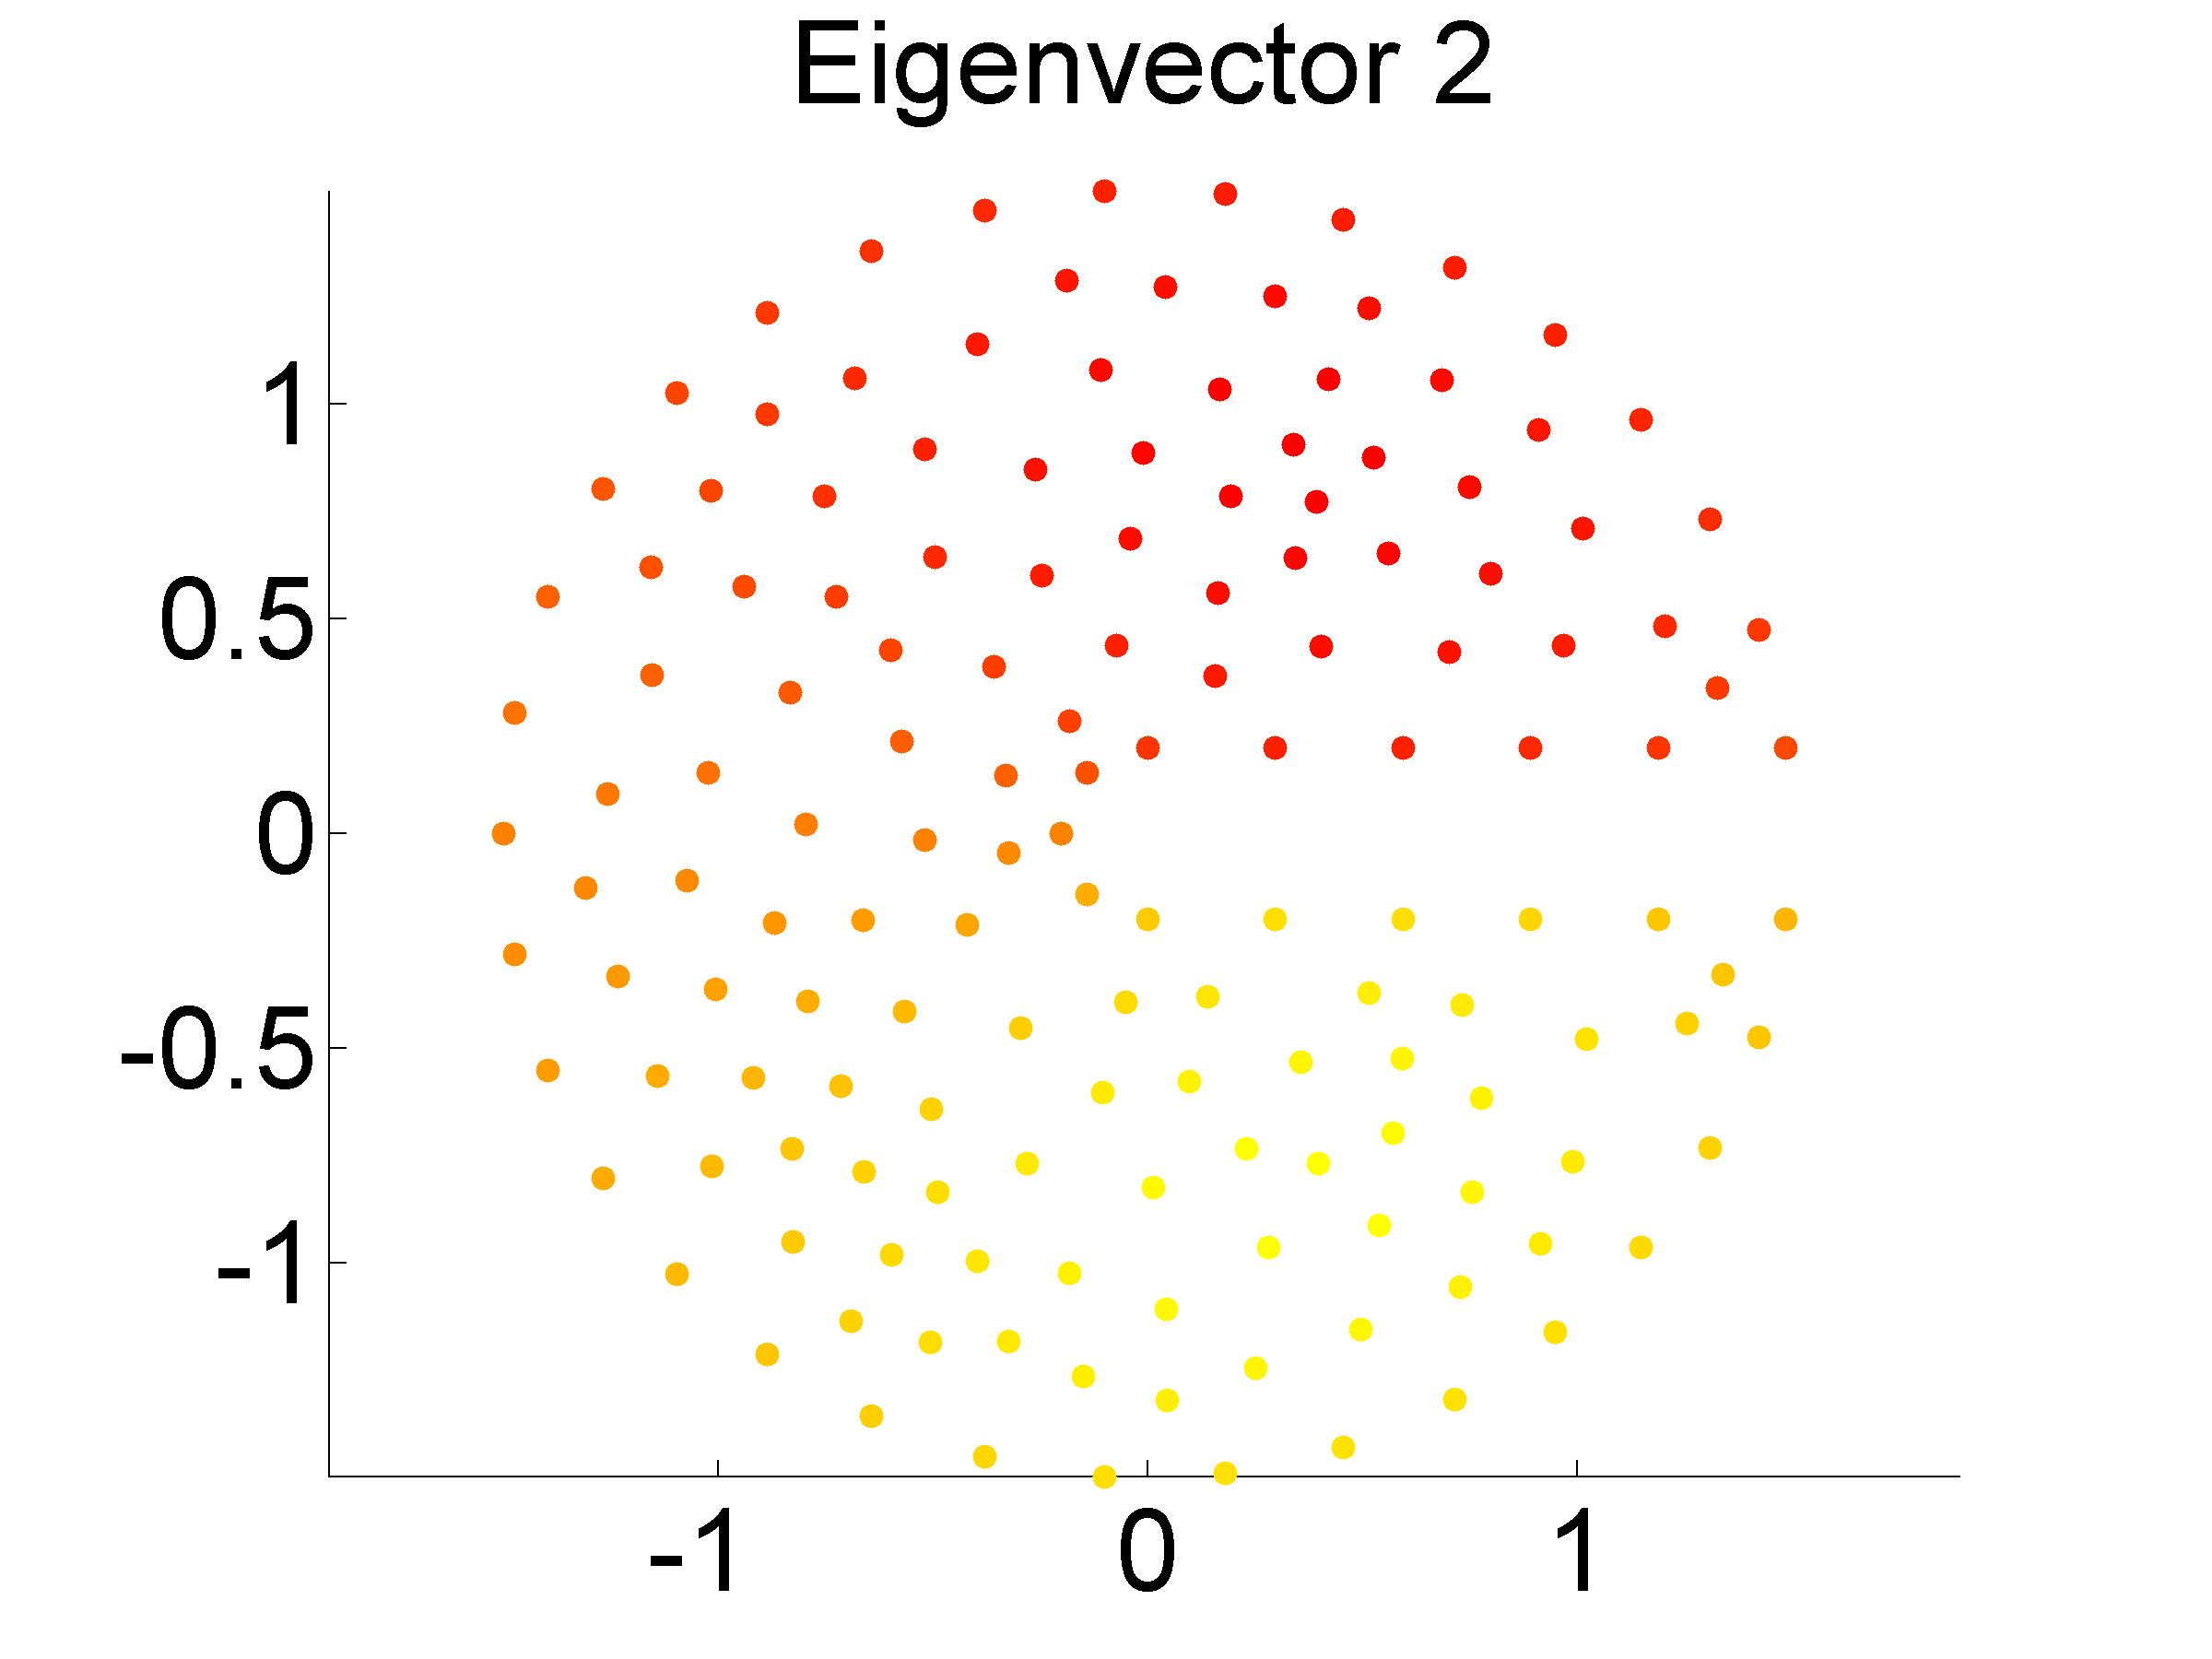
\includegraphics[width=0.18\textwidth]{circle_evec1.jpg}
    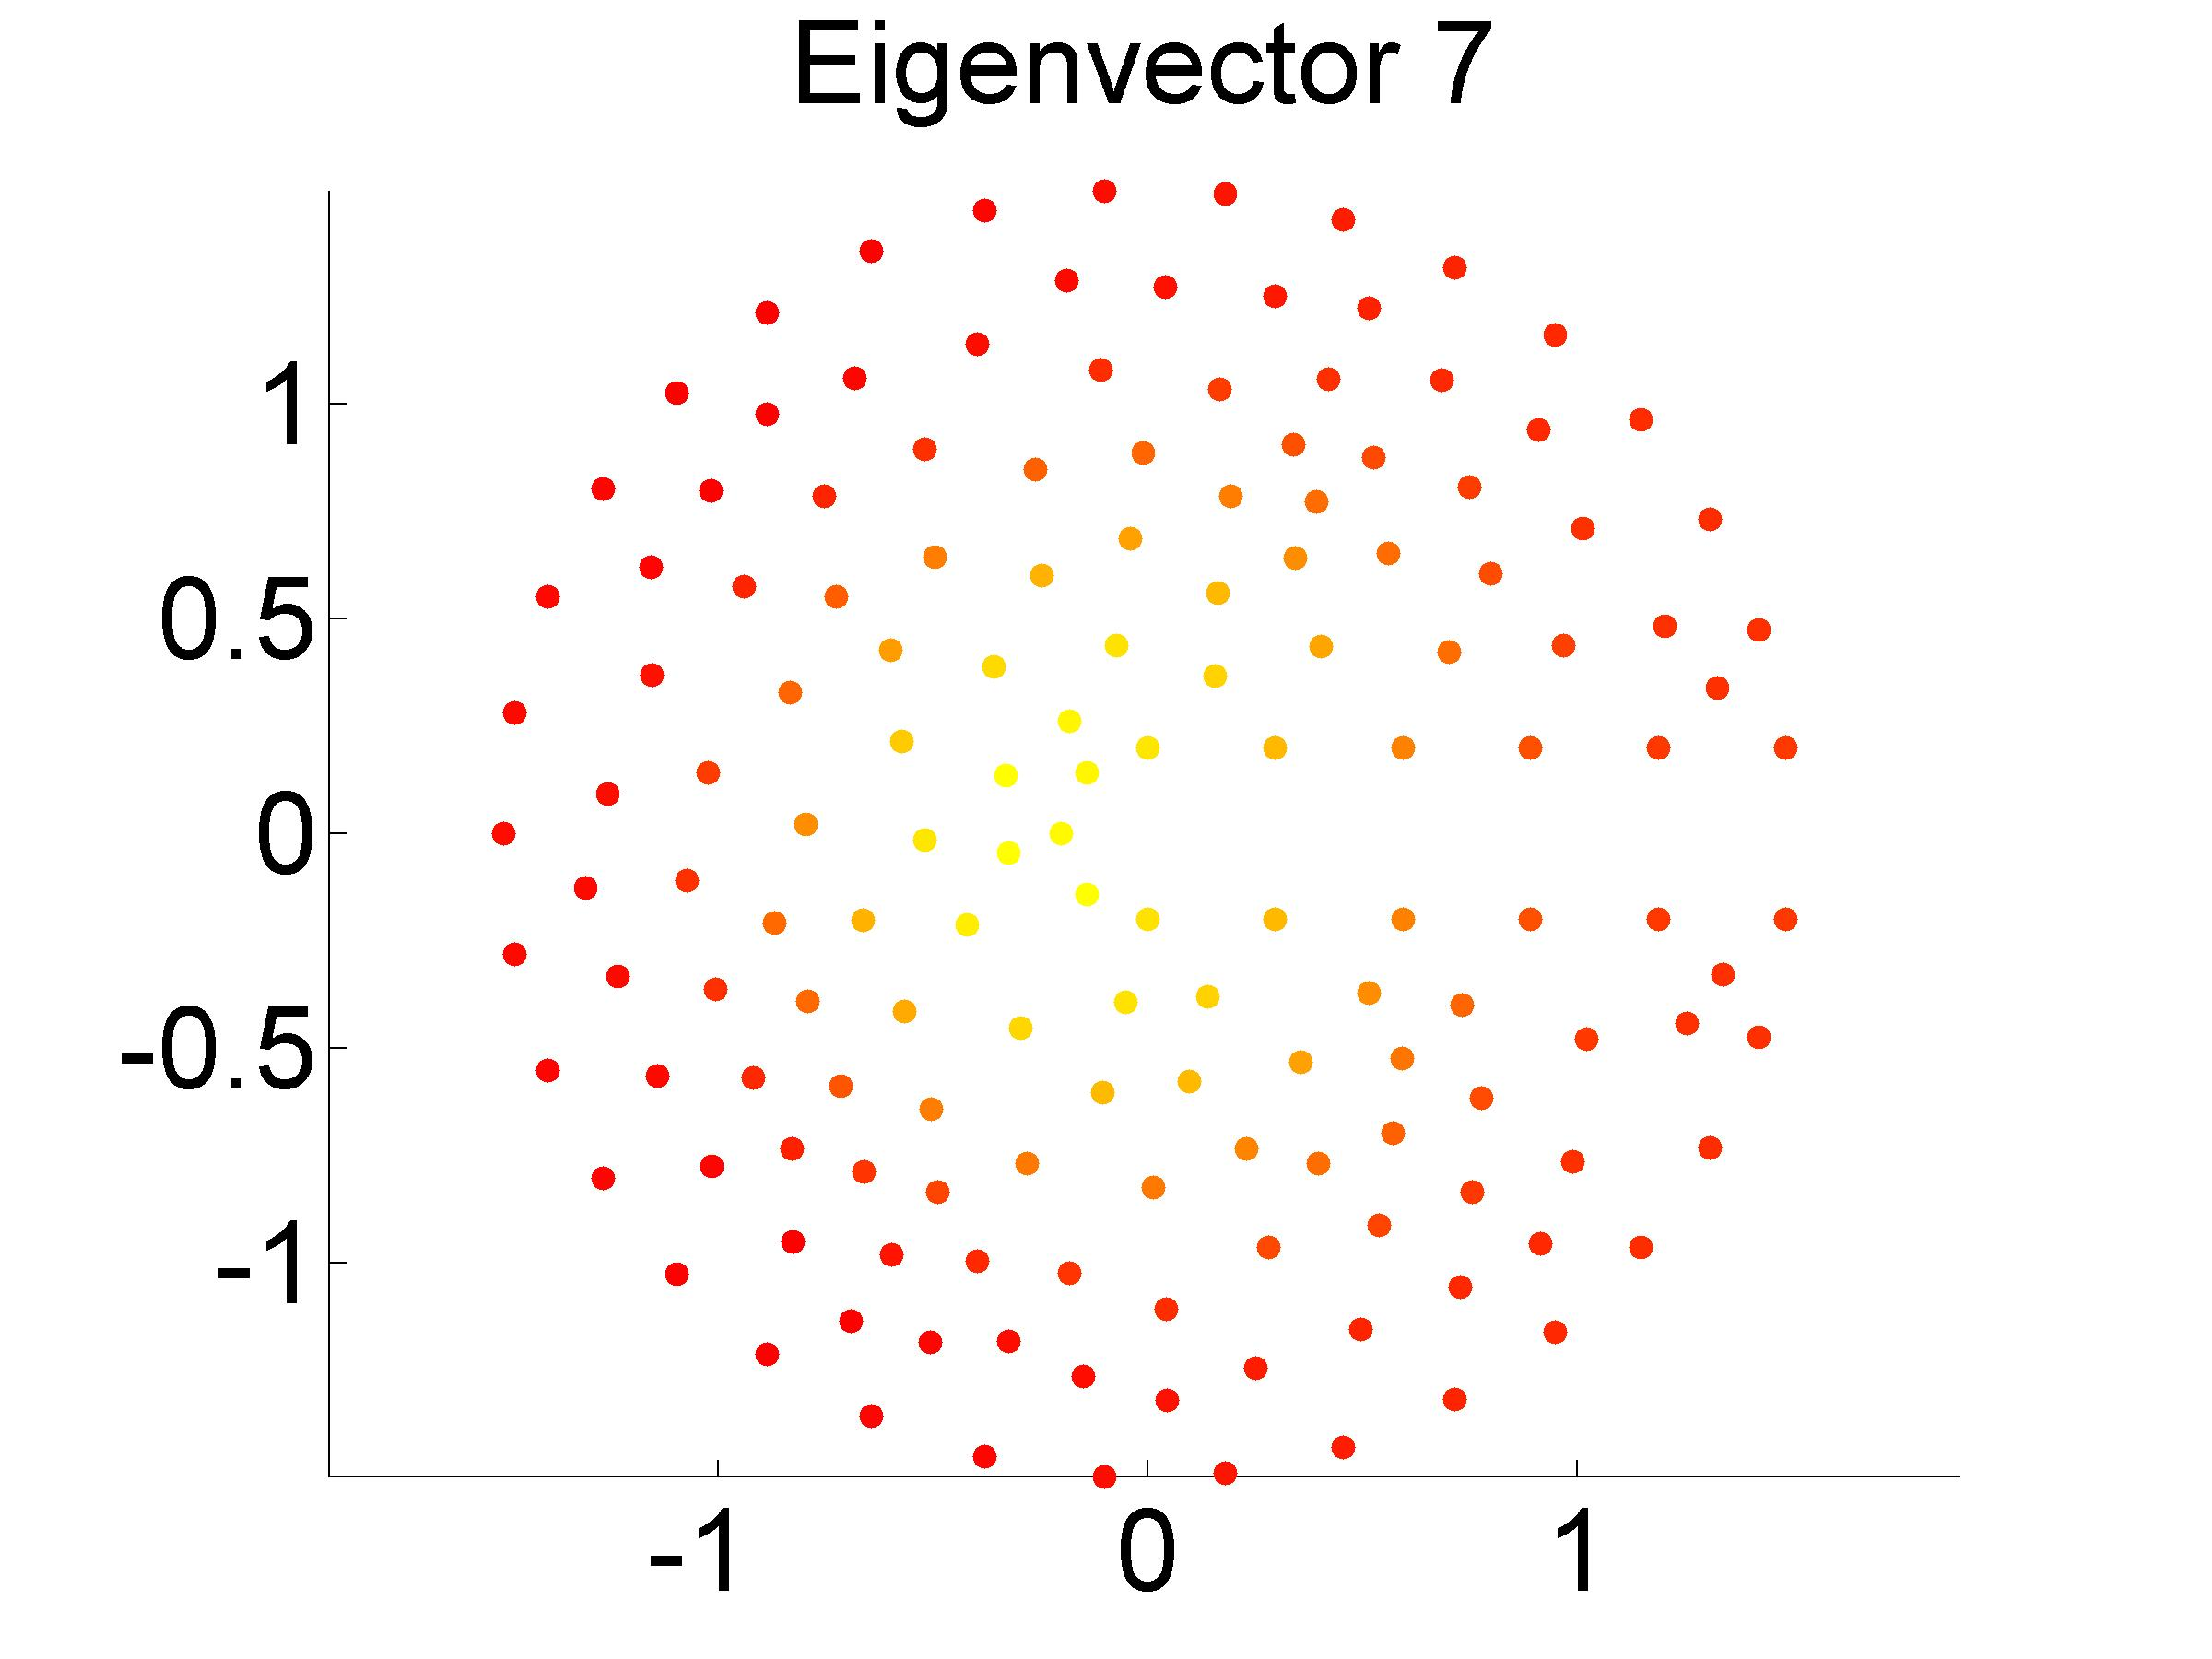
\includegraphics[width=0.18\textwidth]{circle_evec6.jpg}\\

    \vspace{0.05in}

    {\small Diffusion maps approximates the eigenfunctions for a manifold \\ using data sampled from the manifold \par}

\end{frame}

\begin{frame}{DMAPS Implementation }

	\footnotetext{Coifman {\em et al}, PNAS, 2005}
	{\small
    \begin{itemize}
        \item Assume we have data $x_1, x_2, \dots, x_n \in \mathbb{R}^d$ that are sampled 		\\from an underlying manifold $\mathcal{M}$
        \item We have a {\bf distance metric} $d(x_i, x_j)$ for our data
        \item We construct the matrix $W \in \mathbb{R}^{n \times n}$, with
        $$W_{ij} = \exp \left( -\frac{d^2 (x_i, x_j)}{\epsilon} \right) $$
        where $\epsilon$ is a characteristic distance 
        \leavevmode\makebox(0,0){\put(60, 70){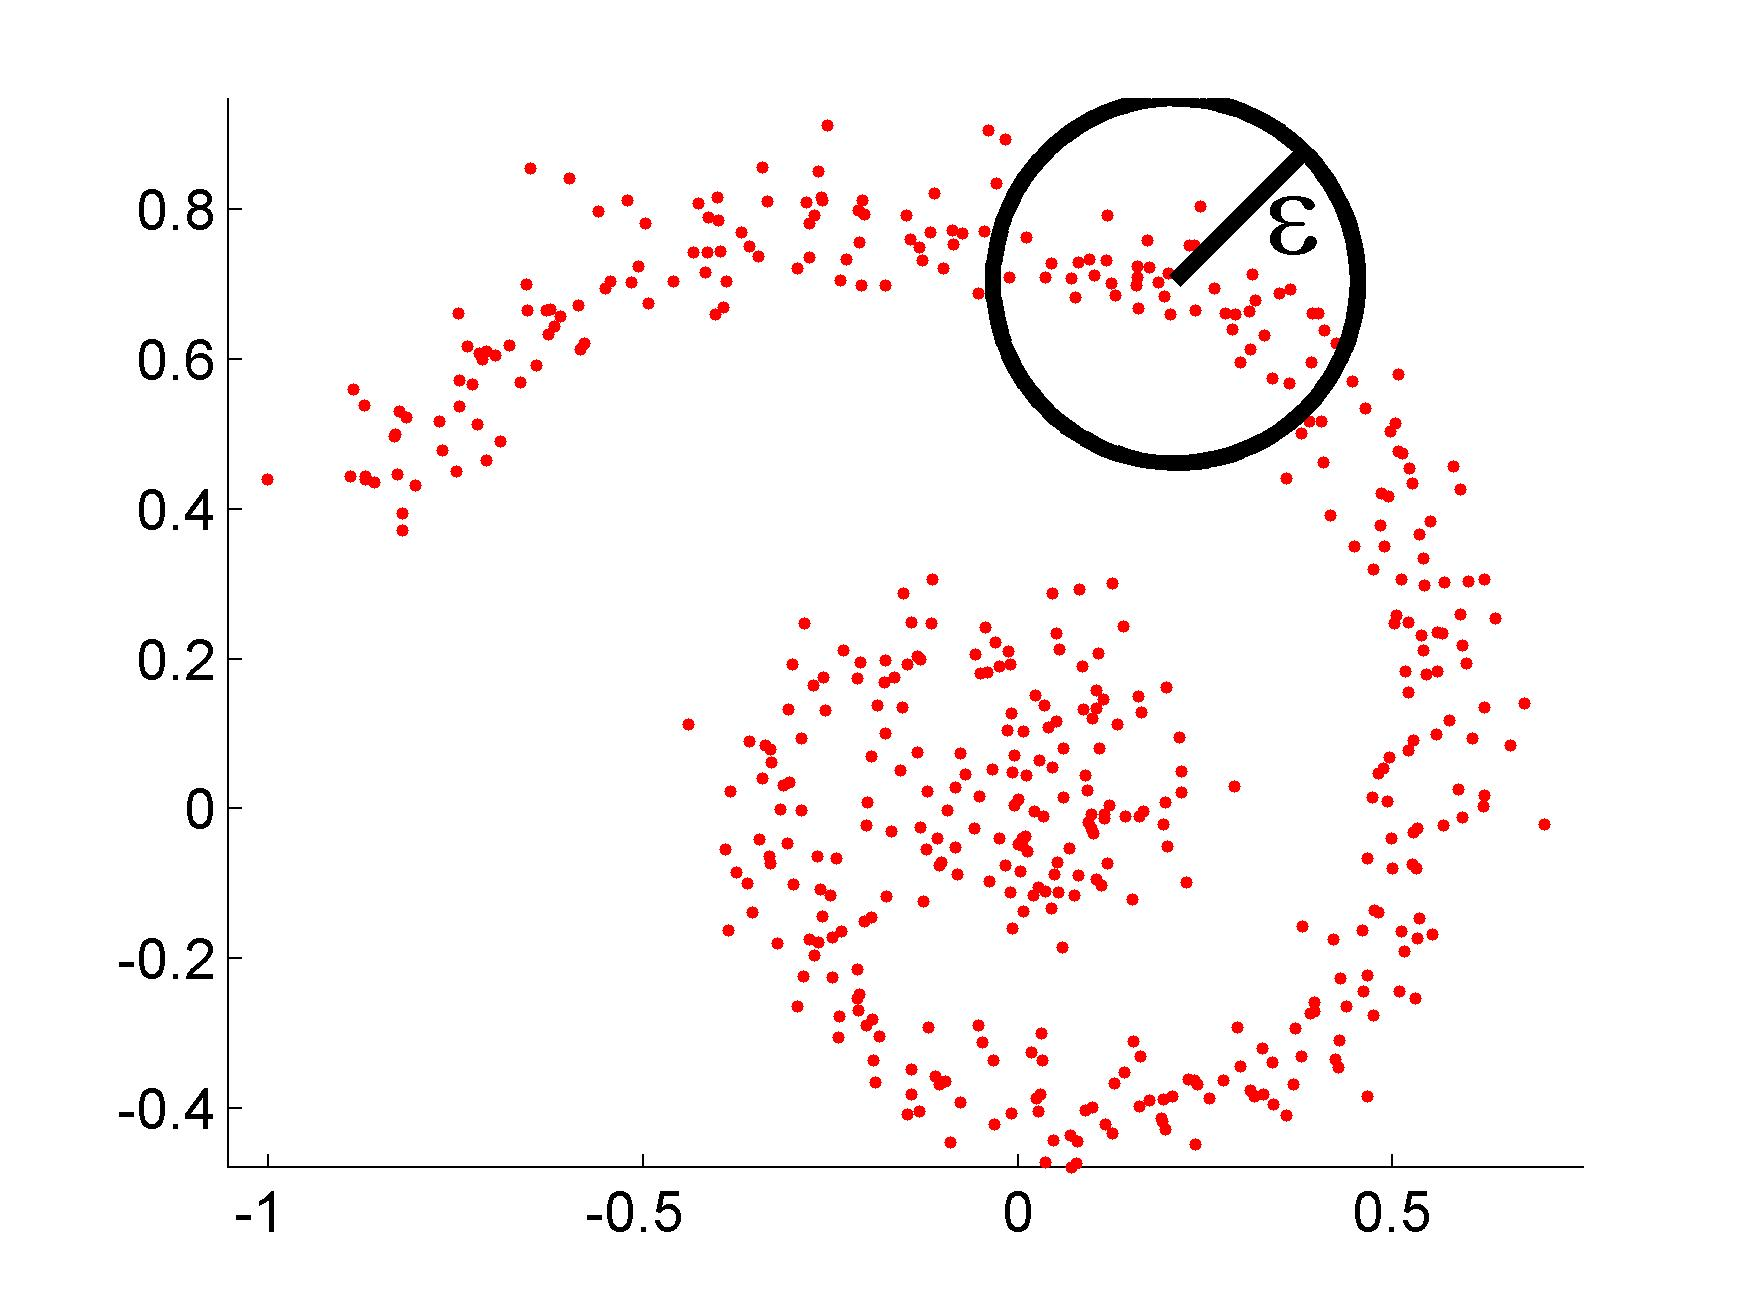
\includegraphics[width=0.25\textwidth]{spiral_with_ball.jpg}}}

        \item We define the diagonal matrix $D$ with $D_{ii} = \sum_{j=1}^{n} W_{ij}$, \\
        and the matrix $A =  D^{-1} W$, where $A$ is a Markov transition matrix

        \item $I-A$ then approximates the Laplacian on the manifold $\mathcal{M}$

        \item We compute the {\em real} {\bf eigenvectors} $\varphi_1, \varphi_2, \dots, \varphi_n$ and \\{\bf eigenvalues} $\lambda_1, \lambda_2, \dots, \lambda_n$ of $A$

        %\item We {\bf order} the eigenvector/eigenvalue pairs such that $|\lambda_1| \ge |\lambda_2| \ge \dots \ge |\lambda_n|$

        \item The eigenvectors then approximate the eigenfunctions \\of the Laplacian {\em on the manifold} $\mathcal{M}$
    \end{itemize}
	\par}

\end{frame}

\begin{frame}{Data-Driven Reduction for Multiscale Data}

{\bf Issue:} Direction of largest variance is not necessarily the {\em slow} direction

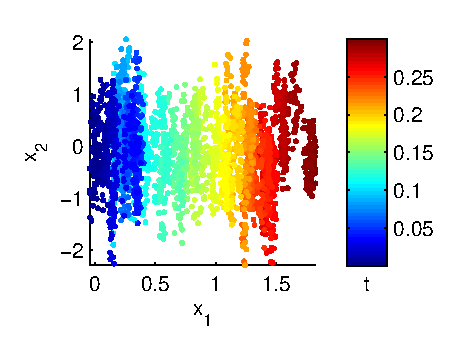
\includegraphics[width=0.5\textwidth]{data_init}
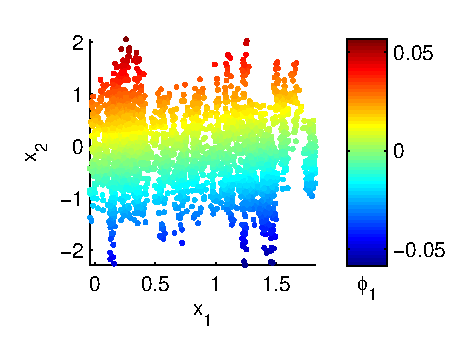
\includegraphics[width=0.5\textwidth]{data_linear_DMAPS}

We will construct a {\em more informative metric} which captures the relative time scales in the data

\end{frame}

\begin{frame}{Mahalanobis Distance: A Good Metric}

We define the Mahalanobis distance, $\| \cdot \|_M$, as
$$\| \vec{x}(t_2) - \vec{x}(t_1) \|^2_M = \| \vec{z}(t_2) - \vec{z}(t_1) \|^2_2$$
where $\vec{z}$ obey the following SDEs
$$dz_i(t) = b_i(\vec{z}(t)) dt + dW_i(t)$$


For the original multiscale SDE we were considering,
\begin{equation*}
\begin{aligned}
dx_i(t) &= a_i(\vec{x}(t)) dt + dW_i(t), & \: 1 \le i \le m \\
dx_i(t) &= \frac{a_i(\vec{x}(t))}{\epsilon} dt + \frac{1}{\sqrt{\epsilon}} dW_i(t) , & \: m+1 \le i \le n
\end{aligned}
\end{equation*}
this amounts to rescaling $\vec{x}_{m+1}, \dots, \vec{x}_n$  by $\sqrt{\epsilon}$. 


\end{frame}

\begin{frame}{Mahalanobis Distance Collapses Fast Directions}

Therefore, we have

\begin{equation*}
\begin{aligned} 
\| \vec{z}(t_2) - \vec{z}(t_1) \|^2_2 &= \sum_{i=1}^n \left( z_i(t_2) - z_i(t_1) \right)^2 \\
&= \sum_{i=1}^m  \left( x_i(t_2) - x_i(t_1) \right)^2 + \sum_{i=m+1}^n \epsilon \left( x_i(t_2) - x_i(t_1) \right)^2
\end{aligned}
\end{equation*}

Fast variables are scaled by $\epsilon$!

\end{frame}


\begin{frame}{Nonlinear Data}

Our data could be obscured by some nonlinear measurement function $\mathbf{f}$. 

\footnotetext{Coifman and Singer, ACHA, 2009}

$$\| \mathbf{f} (\vec{x}(t_2)) - \mathbf{f} (\vec{x}(t_1)) \|^2_M = \| \vec{z}(t_2) - \vec{z}(t_1) \|^2_2 + \mathcal{O}(\|  \mathbf{f} (\vec{x}(t_2)) - \mathbf{f} (\vec{x}(t_1)) \|^4_2)$$

Mahalanobis distance is invariant (to fourth order) to nonlinear transformations!

\end{frame}

\section{Error Analysis}

\begin{frame}{General Error Terms}


\end{frame}

\begin{frame}{Errors from Taylor Expansion}

By Taylor expansion of $\mathbf{g}(y)$ around $\vec{y}(t_1)$ and $\vec{y}(t_2)$ and averaging the two expansions,
%
\begin{equation}
\begin{aligned}
\| \vec{z}(t_2) - \vec{z}(t_1) \|^2_2 =&
\frac{1}{2} \left(\vec{y}(t_2)-\vec{y}(t_1)\right)^T \left(C^\dagger (\vec{y}(t_1)) + C^\dagger (\vec{y}(t_2)) \right) (\vec{y}(t_2)-\vec{y}(t_1)) \\
&+ E_M \left(\vec{y}(t_1), \vec{y}(t_2) \right) \\
&+ \mathcal{O} \left(\| \vec{y}(t_2) - \vec{y}(t_1) \|^6_2 \right)
\end{aligned}
\end{equation}


\begin{equation}
\begin{aligned} 
E_M\left( \vec{y}(t_1), \vec{y}(t_2) \right)
 =
\frac{1}{2} \sum_{i=1}^n \sum_{jkl=1}^{d} &
\left( g_{i, (j)} (\vec{y}(t_1)) g_{i, (k,l)} (\vec{y}(t_1)) -  g_{i, (j)} (\vec{y}(t_2)) g_{i, (k,l)} (\vec{y}(t_2)) \right) \\
& (\vec{y}_j(t_2) - \vec{y}_j(t_1))   (\vec{y}_k(t_2) - \vec{y}_k(t_1))(\vec{y}_l(t_2) - \vec{y}_l(t_1)) \\
+ \frac{1}{8} \sum_{i=1}^n \sum_{jklm=1}^d  &
\left( g_{i, (j,k)} (\vec{y}(t_1)) g_{i, (l,m)} (\vec{y}(t_1)) +  g_{i, (j,k)} (\vec{y}(t_2)) g_{i, (l,m)} (\vec{y}(t_2)) \right) \\
&(\vec{y}_j(t_2) - \vec{y}_j(t_1))  (\vec{y}_k(t_2) - \vec{y}_k(t_1))(\vec{y}_l(t_2) - \vec{y}_l(t_1)) (\vec{y}_m(t_2) - \vec{y}_m(t_1)) \\
+ \frac{1}{6} \sum_{i=1}^n \sum_{jklm=1}^d &
\left( g_{i, (j)} (\vec{y}(t_1)) g_{i, (k,l,m)} (\vec{y}(t_1)) +  g_{i, (j)} (\vec{y}(t_2)) g_{i, (k,l,m)} (\vec{y}(t_2)) \right) \\
& (\vec{y}_j(t_2) - \vec{y}_j(t_1))  (\vec{y}_k(t_2) - \vec{y}_k(t_1))(\vec{y}_l(t_2) - \vec{y}_l(t_1))(\vec{y}_m(t_2) - \vec{y}_m(t_1))
\end{aligned}
\end{equation}
%
where
%
\begin{equation}
\begin{aligned}
g_{i,(j)} &= \sqrt{e_i} \frac{\partial g_i}{\partial y_j}
\\
g_{i,(j,k)} &= \sqrt{e_i}  \frac{\partial^2 g_i}{\partial y_j \partial y_k}
\\
g_{i,(j,k,l)} &= \sqrt{e_i}  \frac{\partial^3 g_i}{\partial y_j \partial y_k \partial y_l}
\end{aligned}
\end{equation}

\end{frame}

\begin{frame}{Errors from covariance estimation}

By It\={o}-Taylor expansion of $\mathbf{f}$ and $\vec{x}(t)$,
\begin{equation}\label{eq:estimated_cov}
\begin{aligned}
\hat{C}_{ij} (\vec{x}_t, \delta t)
=&
\frac{1}{\delta t} \left( \mathbb{E} \left[ y_i (t+\delta t) y_j (t+ \delta t) \mid \vec{y}(t) \right]
- \mathbb{E} \left[ y_i (t+\delta t) \mid \vec{y}(t) \right] \mathbb{E} \left[ y_j (t+\delta t) \mid \vec{y}(t) \right] \right)
\\
=& \sum_{k=1}^n \frac{1}{e_k} \left. \frac{\partial f_{i}}{\partial x_k} \right|_{\vec{x}(t)} \left. \frac{\partial f_{j}}{\partial x_k} \right|_{\vec{x}(t)}
+ E_{C, ij} (\vec{x}(t), \delta t) + \mathcal{O}(\delta t^{3/2})
%=& \sum_{k=1}^n \frac{1}{e_k} \left. \frac{\partial f_{i}}{\partial x_k} \right|_{\vec{x}(t)} \left. \frac{\partial f_{j}}{\partial x_k} \right|_{\vec{x}(t)} \\
%&+ \frac{1}{\delta t} \sum_{k=1}^n f_{i,(k)}(\vec{x}(t)) \left( \mathbb{E} \left[ \int_t^{t+\delta t} \int_{s_1}^{t+\delta t} f_{j,(k,0)}(\vec{x}(s_2)) ds_2 ds_1 \right]
%+ \mathbb{E} \left[  \int_t^{t+\delta t} \int_t^{s_2} f_{j,(0,k)}(\vec{x}(s_1)) ds_1 ds_2\right] \right) \\
%&+  \frac{1}{\delta t} \sum_{k=1}^n f_{j,(k)}(\vec{x}(t)) \left( \mathbb{E} \left[ \int_t^{t+\delta t} \int_{s_1}^{t + \delta t} f_{i,(k,0)}(\vec{x}(s_2)) ds_2 ds_1 \right]
%+ \mathbb{E} \left[ \int_t^{t+\delta t} \int_t^{s_2} f_{i,(0,k)}(\vec{x}(s_1)) ds_1 ds_2 \right] \right) \\
%&+  \frac{1}{\delta t} \sum_{k,l=1}^n \mathbb{E} \left[ \int_t^{t+\delta t}\left( \int_t^{s_2} f_{i,(k,l)}(\vec{x}(s_1)) dW_{s_1, k}  \right) \left(  \int_t^{s_2} f_{j,(k,l)}(\vec{x}(s_1)) dW_{s_1, k} \right) ds_2 \right] \\
%&+ \mathcal{O} (\delta t^{3/2}),
\end{aligned}
\end{equation}
%
where $E_C = \mathcal{O} (\delta t)$ is an error term, with
%
\begin{equation} \label{eq:cov_error}
\begin{aligned}
E_{C, ij} (\vec{x}(t), \delta t) =&
 \frac{1}{\delta t} \sum_{k=1}^n f_{i,(k)}(\vec{x}(t)) \mathbb{E} \left[ \int_t^{t+\delta t} \left( \int_{s_2}^{t+\delta t} f_{j,(k,0)}(\vec{x}(s_1)) ds_1
+ \int_t^{s_2} f_{j,(0,k)}(\vec{x}(s_1)) ds_1 \right) ds_2 \right] \\
&+  \frac{1}{\delta t} \sum_{k=1}^n f_{j,(k)}(\vec{x}(t))  \mathbb{E} \left[ \int_t^{t+\delta t} \left( \int_{s_2}^{t + \delta t} f_{i,(k,0)}(\vec{x}(s_1)) ds_1
+  \int_t^{s_2} f_{i,(0,k)}(\vec{x}(s_1)) ds_1 \right) ds_2 \right] \\
&+  \frac{1}{\delta t} \sum_{k,l=1}^n \mathbb{E} \left[ \int_t^{t+\delta t}\left( \int_t^{s_2} f_{i,(k,l)}(\vec{x}(s_1)) dW_{s_1, k}  \right) \left(  \int_t^{s_2} f_{j,(k,l)}(\vec{x}(s_1)) dW_{s_1, k} \right) ds_2 \right]
\end{aligned}
\end{equation}

\end{frame}

\begin{frame}{Which Parameters to Set?}

\begin{itemize}
\item Kernel scale $\sigma_{kernel}$
\item Time scale used to estimate covariance $\delta t$
\end{itemize}
\end{frame}

\begin{frame}{Setting the Kernel Scale}

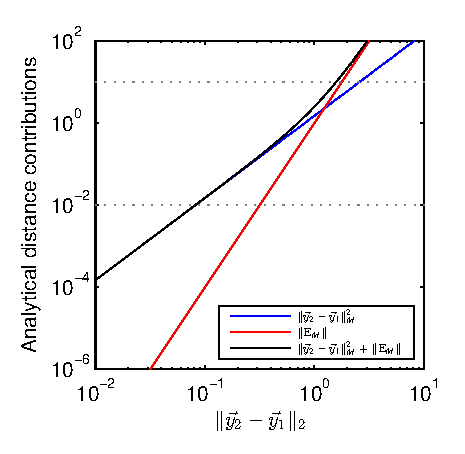
\includegraphics[width=0.5\textwidth]{dist_dy_analytical_nonlinear}

%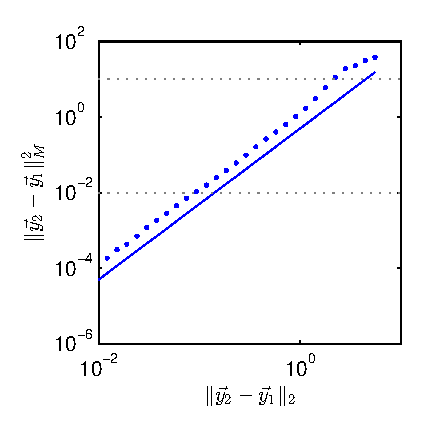
\includegraphics[width=0.5\textwidth]{dist_dy_nonlinear}

\end{frame}

\begin{frame}{Setting the Covariance Timescale}

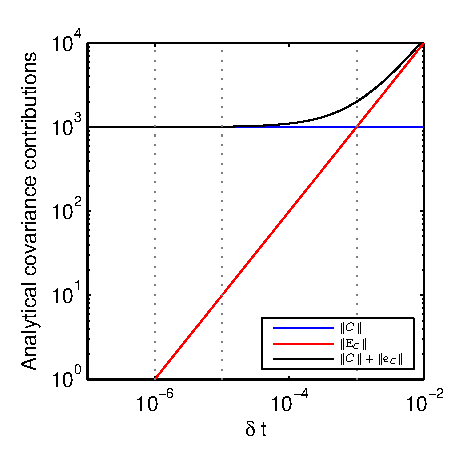
\includegraphics[width=0.5\textwidth]{C_dt_analytical_linear}

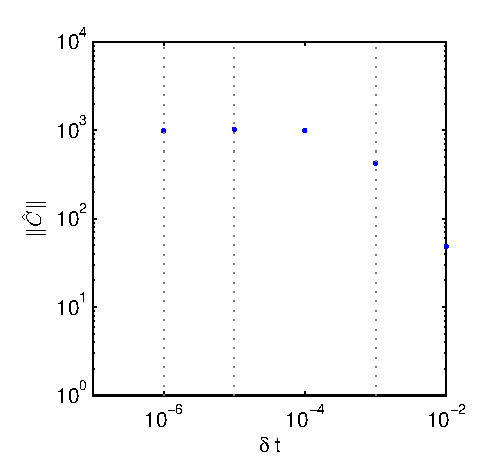
\includegraphics[width=0.5\textwidth]{C_dt_linear}

\end{frame}

\section{Examples}

\begin{frame}{Linear Two-Dimensional Data}

\begin{equation*} 
\begin{aligned}
dx_1(t) &=& 3dt &+& dW_1(t)\\
dx_2(t) &=& -\frac{x_2(t)}{\epsilon} dt &+& \frac{1}{\sqrt{\epsilon}} dW_2(t)
\end{aligned}
\end{equation*} 
where we take $\epsilon = 10^{-3}$

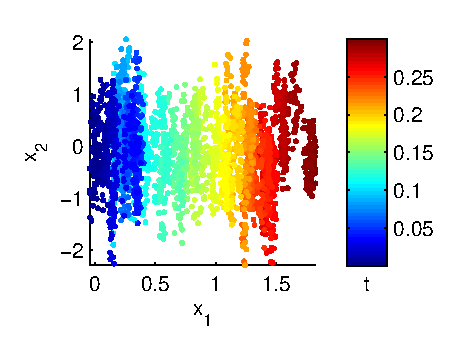
\includegraphics[width=0.5\textwidth]{data_init}
\end{frame}

\begin{frame}{Analysis of data}

\end{frame}

\begin{frame}{Curved ``Half-Moon'' Data}

\end{frame}

\section{Conclusions}

\begin{frame}{Conclusions}

\end{frame}

\end{document}

